\documentclass[11pt]{article}

\usepackage[a4paper]{geometry}
\geometry{left=2.0cm,right=2.0cm,top=2.5cm,bottom=2.5cm}

\usepackage{ctex} % 支持中文的LaTeX宏包
\usepackage{amsmath,amsfonts,graphicx,subfigure,amssymb,bm,amsthm,mathrsfs,mathtools,breqn} % 数学公式和符号的宏包集合
\usepackage{algorithm,algorithmicx} % 算法和伪代码
\usepackage[noend]{algpseudocode} % 算法和伪代码
\usepackage{fancyhdr} % 自定义页眉页脚
\usepackage[framemethod=TikZ]{mdframed} % 创建带边框的框架
\usepackage{fontspec} % 字体设置
\usepackage{adjustbox} % 调整盒子大小
\usepackage{fontsize} % 设置字体大小
\usepackage{tikz,xcolor} % 绘制图形和使用颜色
\usepackage{multicol} % 多栏排版
\usepackage{multirow} % 表格中合并单元格
\usepackage{pdfpages} % 插入PDF文件
\usepackage{listings} % 在文档中插入源代码
\usepackage{wrapfig} % 文字绕排图片
\usepackage{bigstrut,multirow,rotating} % 支持在表格中使用特殊命令
\usepackage{booktabs} % 创建美观的表格
\usepackage{circuitikz} % 绘制电路图
\usepackage{zhnumber} % 中文序号(用于标题)
\usepackage{tabularx} % 表格折行
\usepackage{float} % 图片插入
\usepackage{longtable} % 长表格

\definecolor{dkgreen}{rgb}{0,0.6,0}
\definecolor{gray}{rgb}{0.5,0.5,0.5}
\definecolor{mauve}{rgb}{0.58,0,0.82}
\lstset{
  frame=tb,
  aboveskip=3mm,
  belowskip=3mm,
  showstringspaces=false,
  columns=flexible,
  framerule=1pt,
  rulecolor=\color{gray!35},
  backgroundcolor=\color{gray!5},
  basicstyle={\small\ttfamily},
  numbers=none,
  numberstyle=\tiny\color{gray},
  keywordstyle=\color{blue},
  commentstyle=\color{dkgreen},
  stringstyle=\color{mauve},
  breaklines=true,
  breakatwhitespace=true,
  tabsize=3,
}

% 轻松引用, 可以用\cref{}指令直接引用, 自动加前缀. 
% 例: 图片label为fig:1
% \cref{fig:1} => Figure.1
% \ref{fig:1}  => 1
\usepackage[capitalize]{cleveref}
% \crefname{section}{Sec.}{Secs.}
\Crefname{section}{Section}{Sections}
\Crefname{table}{Table}{Tables}
\crefname{table}{Table.}{Tabs.}

% \setmainfont{Palatino Linotype.ttf}
% \setCJKmainfont{SimHei.ttf}
% \setCJKsansfont{Songti.ttf}
% \setCJKmonofont{SimSun.ttf}
\punctstyle{kaiming}
% 偏好的几个字体, 可以根据需要自行加入字体ttf文件并调用

\renewcommand{\emph}[1]{\begin{kaishu}#1\end{kaishu}}

% 对 section 等环境的序号使用中文
\renewcommand \thesection{\zhnum{section}、}
\renewcommand \thesubsection{\arabic{subsection}}


%%%%%%%%%%%%%%%%%%%%%%%%%%%
%改这里可以修改实验报告表头的信息
\newcommand{\name}{陈琛、王荦璠、张钧玮}
\newcommand{\studentNum}{80}
\newcommand{\major}{计算机科学与技术}
\newcommand{\labNum}{3}
\newcommand{\labName}{添加用户态指令设计专题}
%%%%%%%%%%%%%%%%%%%%%%%%%%%

\begin{document}
\begin{center}
  \LARGE \bf 中国科学院大学 \\《计算机体系结构(研讨课)》实验报告
\end{center}

\begin{center}
  \emph{姓名} \underline{\makebox[12em][c]{\name}} 
  \emph{箱子号} \underline{\makebox[7em][c]{\studentNum}}
  \emph{专业} \underline{\makebox[15em][c]{\major}}\\
  \emph{实验项目编号} \underline{\makebox[3em][c]{\labNum}}
  \emph{实验名称} \underline{\makebox[30em][c]{\labName}}\\
\end{center}

\section{实验任务}

本次实验的目标是在已有的简单流水线CPU基础上,添加更多的普通用户态指令。具体需要实现:

\begin{itemize}
\item 算术逻辑运算类指令。包括slti、sltui、andi、ori、xori、sll、srl、sra以及pcaddu12i。
\item 乘除运算类指令。包括mul.w、mulh.w、mulh.wu、div.w、mod.w、div.wu和mod.w。
\item 转移指令。包括blt、bge、bltu和bgeu。
\item 访存指令的扩展。包括ld.b、ld.h、ld.bu、ld.hu、st.b和st.h。
\end{itemize}

\begin{table}[H]
\centering
\caption{新增指令分类}
\label{tab:new_instructions}
\begin{tabular}{|l|l|}
\hline
\textbf{指令类型} & \textbf{指令说明} \\ \hline
算术逻辑运算类 & 包括立即数运算、移位操作及PC相对地址计算等指令 \\ \hline
乘除运算类 & 实现32位整数的乘法和除法运算,支持有符号和无符号操作 \\ \hline
转移指令 & 添加条件分支指令,支持有符号和无符号比较跳转 \\ \hline
访存指令扩展 & 支持字节和半字的加载存储操作,包含符号扩展 \\ \hline
\end{tabular}
\end{table}

\section{设计详细分析}

\subsection{总体设计思路}

在本次实验中,我们采用了模块化的设计方法,将新增指令的实现分为三个层次进行。首先,通过修改指令译码逻辑,添加算术逻辑运算、移位操作、条件分支以及访存指令的译码支持,并完善ALU模块以支持这些操作。其次,设计独立的mul.v和div.v模块,分别实现乘法和除法运算的基本功能。这些模块采用多周期执行的方式,通过移位相加算法实现乘法,通过恢复余数法实现除法,为上层提供了清晰的接口。最后,将独立的乘除法模块集成到流水线CPU中,同时协调新增指令与原有流水线结构的兼容性(核心在于处理乘除法指令的多周期执行特性与流水线单周期推进的矛盾)。

\subsection{处理器结构设计框图}

% \begin{figure}[H]
%   \centering
%   \includegraphics[width=0.8\textwidth]{fig/processor_structure.png}
%   \caption{处理器结构设计框图}
%   \label{fig:processor_structure}
% \end{figure}

\subsection{关键设计模块}

\subsubsection{逻辑运算、转移与访存指令的实现}

\subsubsection{乘除法模块的设计与封装}

为支持 mul.w/mulh.w/mulh.wu 与
div.w/mod.w/div.wu/mod.wu,本项目将乘法与除法拆分为两个独立的多周期运算单元,并通过清晰的握手信号与 EXE 阶段对接。二者均以 32 位宽(可参数化 XLEN=32)为核心数据通道,使用移位-累加与恢复余数两类经典迭代算法,保证硬件资源可控与时序友好。、

\begin{itemize}

\item \textbf{模块接口与时序约束} 

两个模块的基本接口如下(节选接口,省略若干内寄存器与中间连线):
    
\begin{lstlisting}[language=verilog]
// mul.v(32x32 → 64,支持有/无符号)
module mul #(
    parameter XLEN = 32
)(
    input  wire                  clk,
    input  wire                  resetn,
    input  wire                  start,        // 单拍启动脉冲
    input  wire                  signed_mode,  // 1:有符号;0:无符号
    input  wire [XLEN-1:0]       op_a,
    input  wire [XLEN-1:0]       op_b,
    output wire                  busy,         // 运算进行中
    output wire                  done,         // 单次运算完成(脉冲)
    output wire [2*XLEN-1:0]     product       // 64 位乘积
);
\end{lstlisting}
    
\begin{lstlisting}[language=verilog]
// div.v(32/32 → 32 商 + 32 余数,支持有/无符号)
module div #(
    parameter XLEN = 32
)(
    input  wire            clk,
    input  wire            resetn,
    input  wire            start,           // 单拍启动脉冲
    input  wire            signed_mode,     // 1:有符号;0:无符号
    input  wire [XLEN-1:0] dividend,
    input  wire [XLEN-1:0] divisor,
    output wire            busy,            // 运算进行中
    output wire            done,            // 单次运算完成(脉冲)
    output wire            divide_by_zero,  // 除数为 0 标志
    output wire [XLEN-1:0] quotient,        // 商
    output wire [XLEN-1:0] remainder        // 余数
);
\end{lstlisting}
    
start 仅在指令发射到 EXE 的首拍拉高;单元据此锁存操作数并拉高 busy,直至迭代结束拉低 busy、同时产生单拍 done。流水线侧通过 exe\_ready\_go/allowin 与 busy/done 联动,保障多周期期间暂停推进,完成后再释放(对应 3.3 小节的多周期 FSM 控制)。
    
\item \textbf{符号处理与绝对值通道} 
    
两单元均以统一的无符号迭代内核实现有/无符号两种语义。做法是:

1. 在 \texttt{signed\_mode=1} 时,先对被乘数/被除数求绝对值(两数取幅值),内部以无符号路径迭代;

2. 乘法:最终结果的符号由两操作数符号异或得到;若为负,则对 64 位乘积做二进制补码取反加一;

3. 除法:内部先得到无符号的 商|余,最终根据被除数/除数符号恢复商的符号,余数符号与被除数一致(与指令集定义相容);同时在 \texttt{divisor=0} 时置位 \texttt{divide\_by\_zero} 并给出约定结果(实现中为合法的零/保持模式)。

\item \textbf{乘法:移位-部分积累加(Shift–Add)}
    
乘法器采用一位/一拍的移位-累加结构:

$\bullet$ 迭代寄存器:\texttt{acc\_r}(累加器,承载部分积)、\texttt{multiplicand\_r}、\texttt{multiplier\_r} 与 \texttt{count\_r}(循环计数,宽度 \texttt{COUNT\_WIDTH=\$clog2(XLEN)+1} );

$\bullet$ 每拍操作:检查 \texttt{multiplier\_r[0]},若为 1 则 \texttt{acc\_r += multiplicand\_r};随后 \texttt{multiplicand\_r} 左移一位,\texttt{multiplier\_r} 右移一位,\texttt{count\_r--};

$\bullet$ 结束条件:当 \texttt{count\_r==1} 时进入最后一次累加/移位,下一拍置 \texttt{done=1}、\texttt{busy=0},\texttt{product} 输出稳定(含已完成的符号修正)。

该结构每次只做一次 32/64 位加法与移位,时序友好、面积较小;代价是潜在的 32 拍延迟。

\item \textbf{除法:恢复余数法(Restoring Division)}

除法器采用恢复余数法,一拍处理一位,被除数自高位至低位移入:

$\bullet$ 关键寄存器:\texttt{remainder_mag_r}(当前余数幅值)、\texttt{quotient_mag_r}(当前商幅值)、\texttt{dividend_shift_r}(被除数移位源)、\texttt{divisor_mag_r}(除数幅值)、\texttt{count\_r};

$\bullet$ 每拍流程:

\hspace{2em} 1. 余数左移一位并移入 \texttt{dividend\_shift\_r} 的下一位;

\hspace{2em} 2. 试减 \texttt{divisor\_mag\_r} 得到 \texttt{remainder\_sub};

\hspace{2em} 3. 若试减结果非负(\texttt{ge\_candidate}),则记 1(当前位商为 1),余数采纳 \texttt{remainder\_sub};否则当前位商为 0,余数保留;

\hspace{2em} 4. \texttt{count\_r--},直到 \texttt{last\_cycle};

\end{itemize}

\subsubsection{乘除法指令的多周期实现}

首先,将ALU操作码的位宽从原有的12位扩展到19位,以支持新增的乘除法指令。在IDU模块中,修改alu\_op的定义,将乘除法指令编码到高位。具体实现中,alu\_op[12]到alu\_op[18]分别对应mul.w、mulh.w、mulh.wu、div.w、mod.w、div.wu和mod.wu指令:

\begin{lstlisting}[language=verilog]
assign alu_op[12] = inst_mul_w;    // MUL.W: 32x32->32 (low part)
assign alu_op[13] = inst_mulh_w;   // MULH.W: 32x32->32 (high part, signed)
assign alu_op[14] = inst_mulh_wu;  // MULH.WU: 32x32->32 (high part, unsigned)
assign alu_op[15] = inst_div_w;    // DIV.W: signed division
assign alu_op[16] = inst_mod_w;    // MOD.W: signed modulo
assign alu_op[17] = inst_div_wu;   // DIV.WU: unsigned division
assign alu_op[18] = inst_mod_wu;  // MOD.WU: unsigned modulo
\end{lstlisting}

在指令译码方面,添加对乘除法指令类型的识别逻辑如下:

\begin{lstlisting}[language=verilog]
wire ty_MD        = op_31_26_d[0] & op_25_22_d[0] & ((inst[21:18] == 4'b0111) | (inst[21:18] == 4'b1000));
wire inst_mul_w   = ty_MD & op_21_20_d[1] & (inst[17:15] == 3'b000);
wire inst_mulh_w  = ty_MD & op_21_20_d[1] & (inst[17:15] == 3'b001);
wire inst_mulh_wu = ty_MD & op_21_20_d[1] & (inst[17:15] == 3'b010);
wire inst_div_w   = ty_MD & op_21_20_d[2] & (inst[17:15] == 3'b000);
wire inst_mod_w   = ty_MD & op_21_20_d[2] & (inst[17:15] == 3'b001);
wire inst_div_wu  = ty_MD & op_21_20_d[2] & (inst[17:15] == 3'b010);
wire inst_mod_wu  = ty_MD & op_21_20_d[2] & (inst[17:15] == 3'b011);
\end{lstlisting}

在执行阶段,由于乘除法的特殊性,需要设计多周期状态机以及握手机制来处理乘除法指令的执行。这部分工作是乘除法指令实现的核心。首先识别出哪些操作是多周期的:

\begin{lstlisting}[language=verilog]
assign is_mul_op = exe_alu_op[12] | exe_alu_op[13] | exe_alu_op[14];
assign is_div_op = exe_alu_op[15] | exe_alu_op[16] | exe_alu_op[17] | exe_alu_op[18];
assign is_multicycle_op = is_mul_op | is_div_op;
\end{lstlisting}

然后设计状态机来控制流水线的暂停和恢复。状态机通过multicycle\_executing信号来跟踪当前是否正在执行多周期指令:

\begin{lstlisting}[language=verilog]
always @(posedge clk) begin
    if (~resetn) begin
        multicycle_executing <= 1'b0;
    end else begin
        if (start_multicycle) begin
            // Start multi-cycle execution
            multicycle_executing <= 1'b1;
        end else if (multicycle_executing) begin
            // Wait for completion of multi-cycle operation
            if ((is_mul_op & mul_done) | (is_div_op & div_done))
                multicycle_executing <= 1'b0;
        end
    end
end
\end{lstlisting}

流水线的控制逻辑也相应调整,确保在多周期指令执行期间,流水线能够正确暂停:

\begin{lstlisting}[language=verilog]
assign exe_ready_go = ~start_multicycle & ~multicycle_executing;
assign exe_allowin = ~exe_valid | (exe_ready_go & mem_allowin);
assign exe_to_mem_valid = exe_valid & exe_ready_go;
\end{lstlisting}

乘除法模块的启动信号逻辑如下。启动信号只在指令开始执行时维持一个周期:

\begin{lstlisting}[language=verilog]
always @(posedge clk) begin
    if (~resetn) begin
        mul_start <= 1'b0;
        div_start <= 1'b0;
    end else begin
        // Start signal active for one cycle when new multicycle instruction arrives
        mul_start <= is_mul_op & start_multicycle;
        div_start <= is_div_op & start_multicycle;
    end
end
\end{lstlisting}

对于不同的乘除法指令,根据指令类型从乘法或除法的结果中选择正确的数据:

\begin{lstlisting}[language=verilog]
assign final_result = exe_alu_op[12] ? mul_product[31:0] :     // MUL.W: low 32 bits
                      exe_alu_op[13] ? mul_product[63:32] :    // MULH.W: high 32 bits (signed)
                      exe_alu_op[14] ? mul_product[63:32] :    // MULH.WU: high 32 bits (unsigned)
                      exe_alu_op[15] ? div_quotient :          // DIV.W: quotient (signed)
                      exe_alu_op[16] ? div_remainder :         // MOD.W: remainder (signed)
                      exe_alu_op[17] ? div_quotient :          // DIV.WU: quotient (unsigned)
                      exe_alu_op[18] ? div_remainder :         // MOD.WU: remainder (unsigned)
                      exe_alu_result;                          // Regular ALU result
\end{lstlisting}

\section{实验过程中遇到的问题}

\subsection{EXEU多周期流水线信号问题}

\begin{figure}[H]
  \centering
  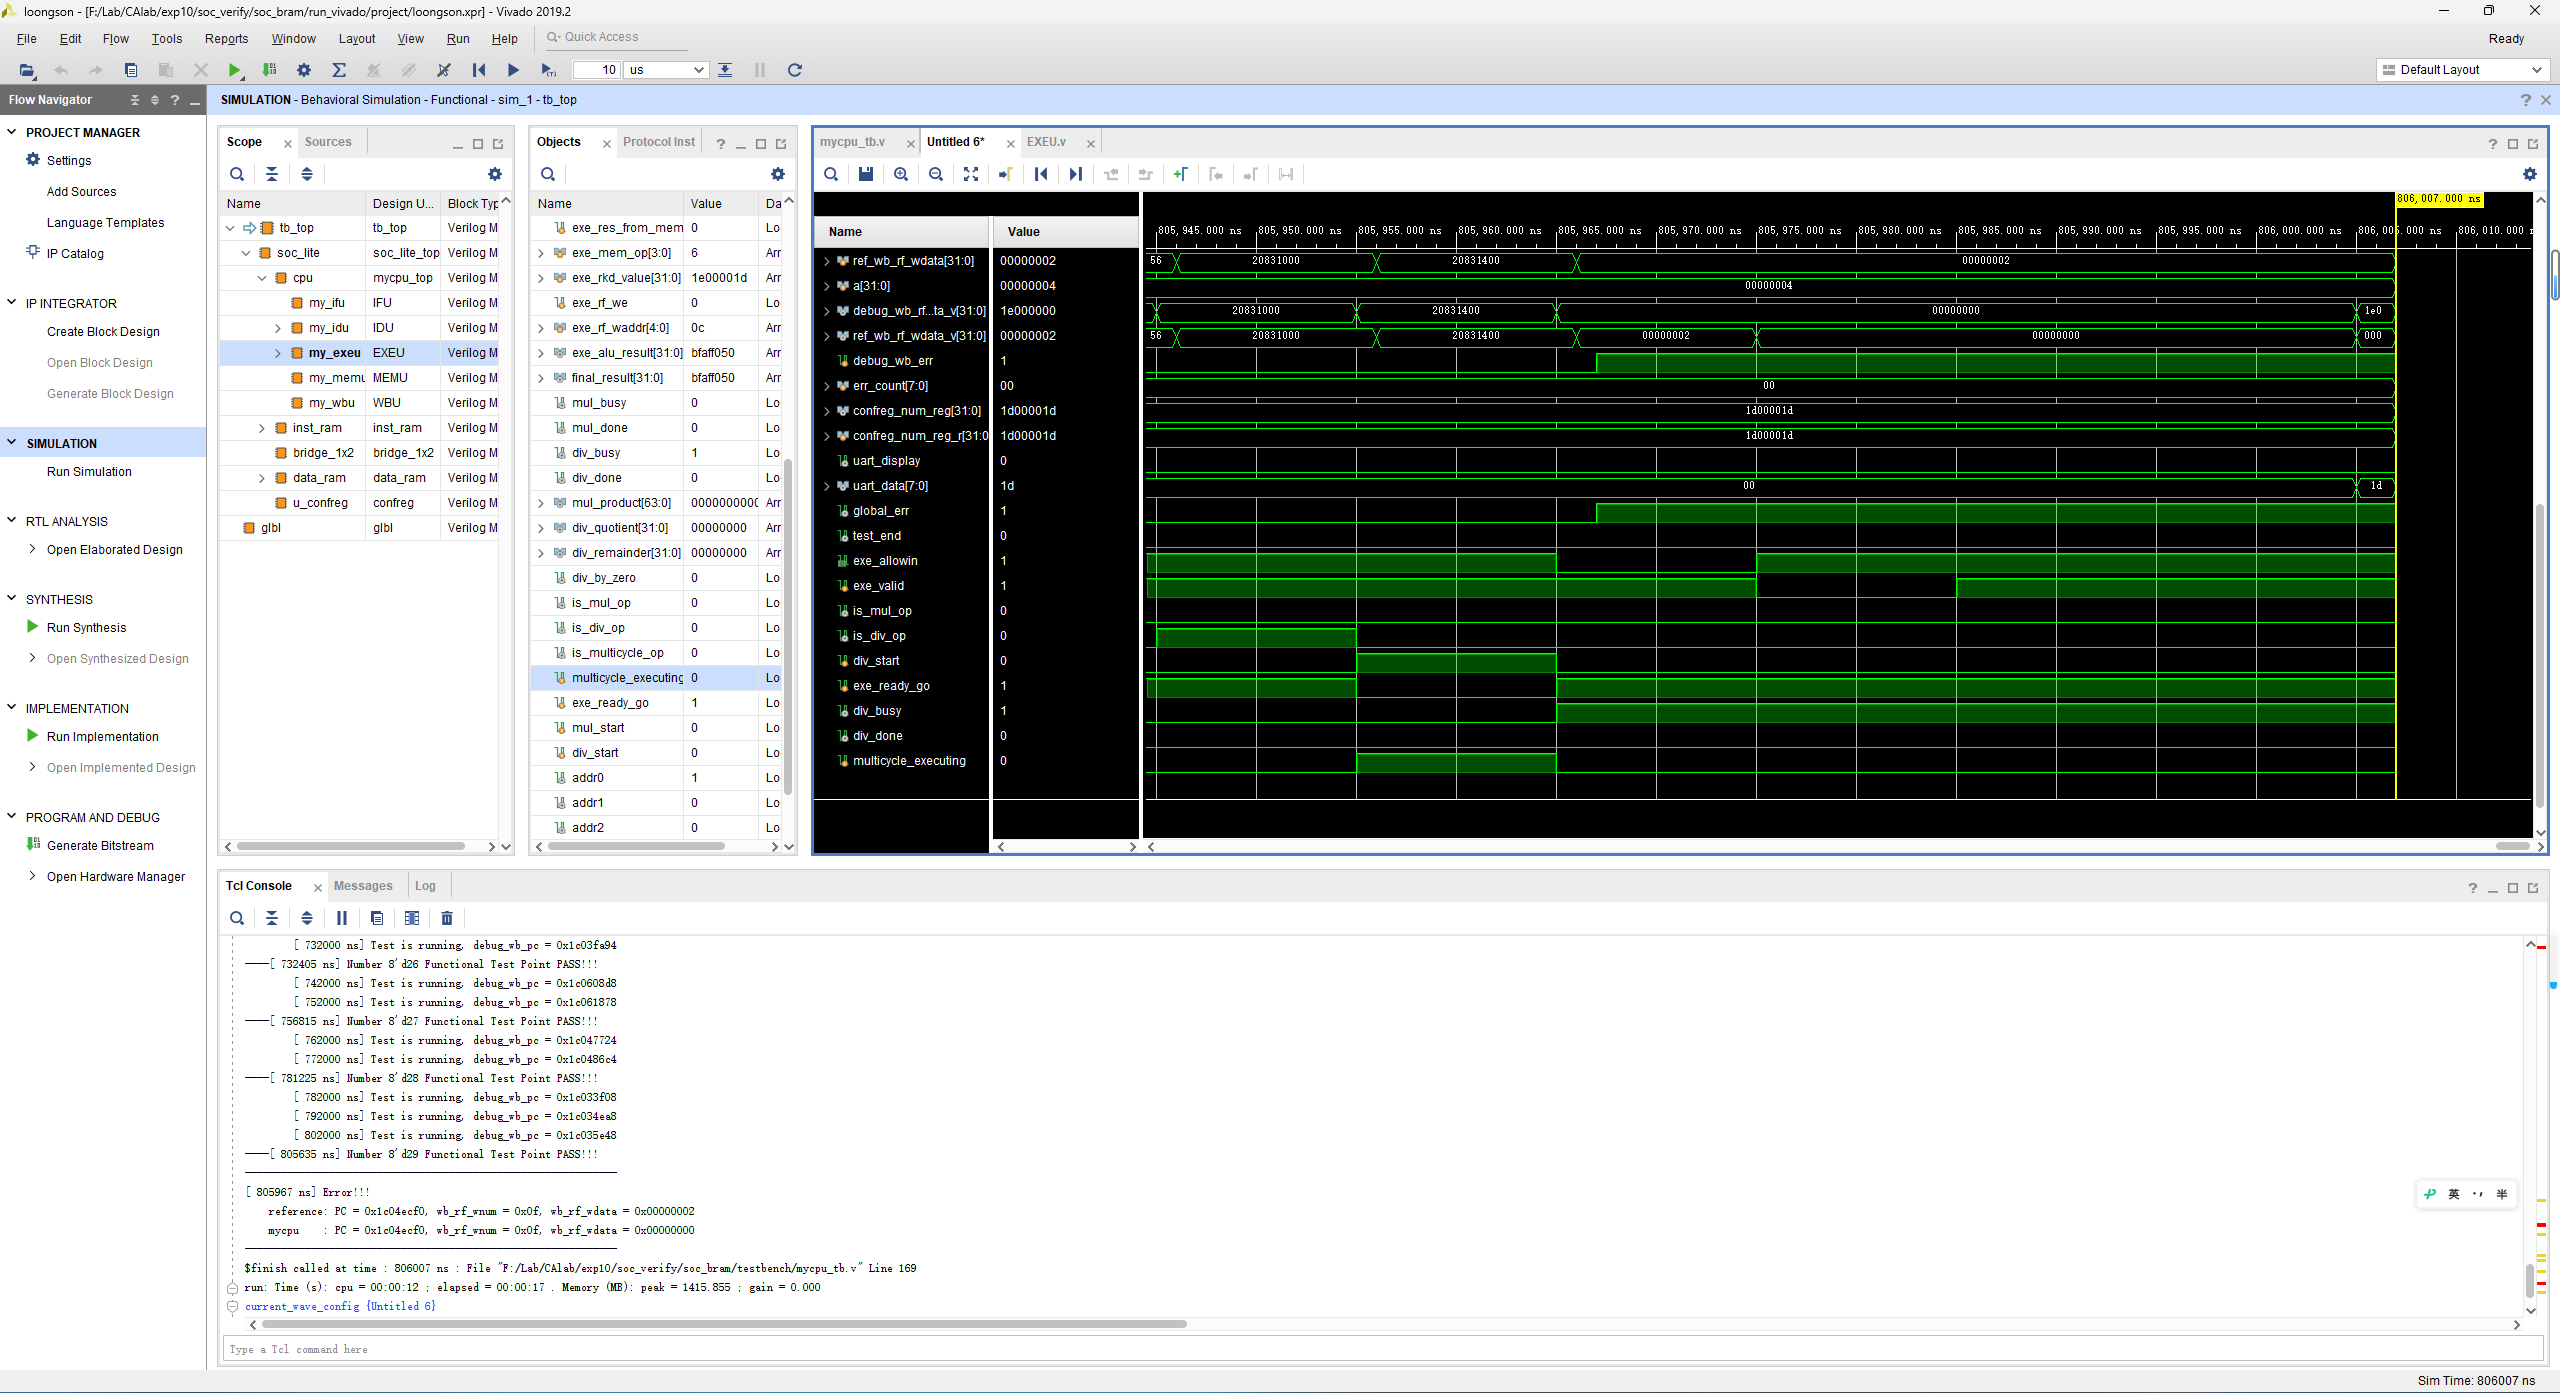
\includegraphics[width=\textwidth]{fig/exeu_multicycle_error.png}
  \caption{EXEU多周期流水线信号问题}
  \label{fig:exeu_multicycle_error}
\end{figure}

在设计多周期EXEU模块的初期,流水线allowin、ready\_go等信号的逻辑频频出错,在波形图中反映为多周期乘除法指令过程中exe阶段的valid、allowin等信号异常,导致与前后流水级的数据传递出现问题。仔细检查代码后发现,多周期下的EXEU不能继续保持原有的ready\_go信号赋值逻辑(由于原先单周期的特性,ready\_go信号始终被设置为1);此外,valid等其他信号均需要根据多周期特性进行重新修正。

为了更好地区分多周期EXEU的执行阶段,同时避免时序逻辑常常“慢一拍”的典型问题,我们引入了start\_exe寄存器,并通过组合逻辑定义start\_multicycle信号,用于标记多周期执行的开始。

\begin{lstlisting}[language=verilog]
reg start_exe;
always @(posedge clk) begin
    if (id_to_exe_valid & exe_allowin) begin
        {exe_alu_op, exe_res_from_mem, exe_alu_src1, exe_alu_src2, exe_mem_op, exe_rf_we, exe_rf_waddr, exe_rkd_value, exe_pc} <= id_to_exe_zip;
        start_exe <= 1'b1;
    end else
        start_exe <= 1'b0;
end
wire   start_multicycle;
assign start_multicycle = is_multicycle_op & start_exe;  // Special time stamp
\end{lstlisting}

此后,根据start\_multicycle信号,便可以正常对流水线控制信号进行赋值(具体见上文设计分析部分,这里不再赘述)。

\subsection{XX问题}

\subsection{XX问题}

\section{实验结果}


所有测试均通过验证,证明了我们实现的CPU能够正确支持所有新增的用户态指令。


\section{小组成员分工}

陈琛:

张钧玮:负责乘除法运算单元的设计与调试,调整运算算法以简化电路确保时序友好。

王荦璠:将乘除法模块集成到流水线CPU中,处理乘除法指令的多周期执行特性与流水线单周期推进的矛盾,协调新增指令与原有流水线结构的兼容性。

\end{document}